%!TEX root = ../ausarbeitung.tex
\section{Klassifizierung mit Spatial Pyramid Matching}

\subsection{Grundidee Spatial Pyramid Matching}

\begin{figure}
	\centering
	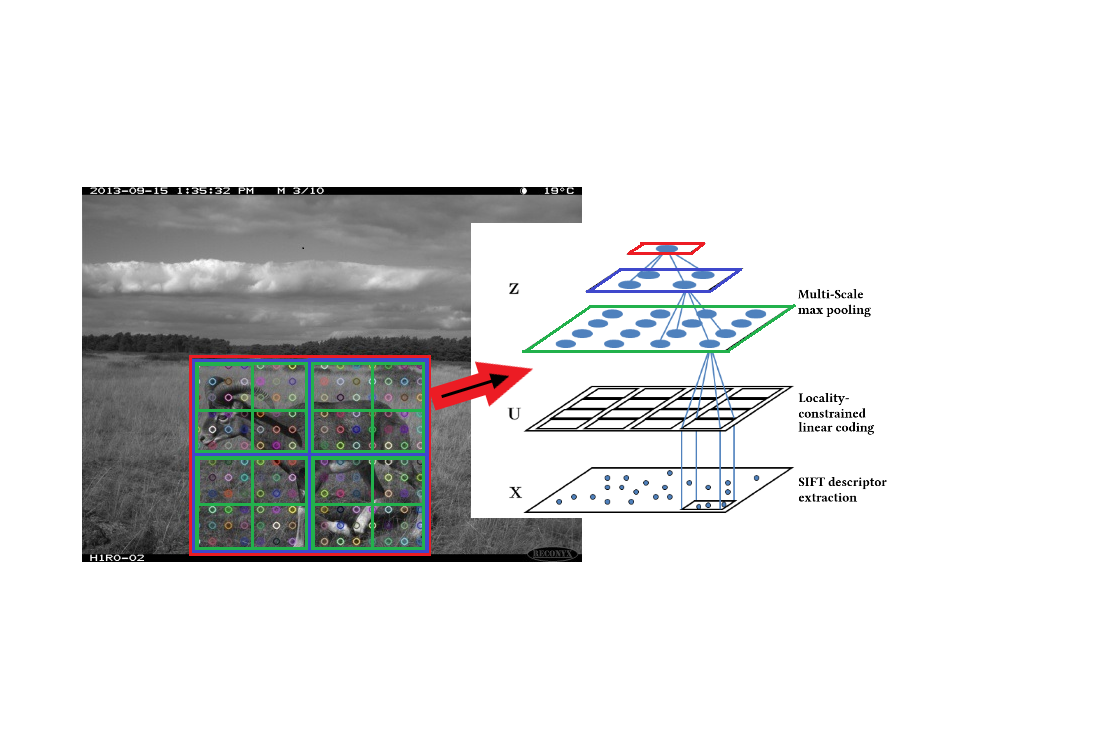
\includegraphics[scale=1]{img/sift_spm.png}
	\caption{Architektur des Algorithmus mit Veranschaulichung der Spatial Pyramid auf SIFT-Features und Pooling. Im Anschluss werden der $L_0$- (rot) und die $L_1$- (blau) und $L_2$-Codes (grün) konkateniert \cite{yygh09}.}
\end{figure}

-hintergrund: Lazebnik et al., Scene Classification
-aufteilung in immer feinere regionen
-bild mit dense features und spatial pyramid einfügen
-features für alle regionen (sift, lbp)
-berechnungen von codes aufgrund dieser features (enkodierung, pooling, normalisierung)
-trainieren einer SVM mit den codes

\subsection{Locality-constrained Linear Coding}

-kurze einleitung
-vortraining des codebooks mit clustering
-vergleich mit vector quantization
-gleichung
-lösungsalgorithmus
-pooling
-normalisierung
-lineare separierarkeit, laufzeit, bezug auf hog kapitel
-kurze erwähnung der svm mit squared-hinge-loss und 

\subsection{Implementierung}

-umsetzung numpy, optimierung numba
-opencv für sift, scikit-image für lbp
-clustering und linear svm mit scikit-learn
-transformer mit scikit-learn, einbettung in pipeline